\begin{center}
\begin{tikzpicture}
    \node[anchor=south west,inner sep=0] (image)  at (0,0) {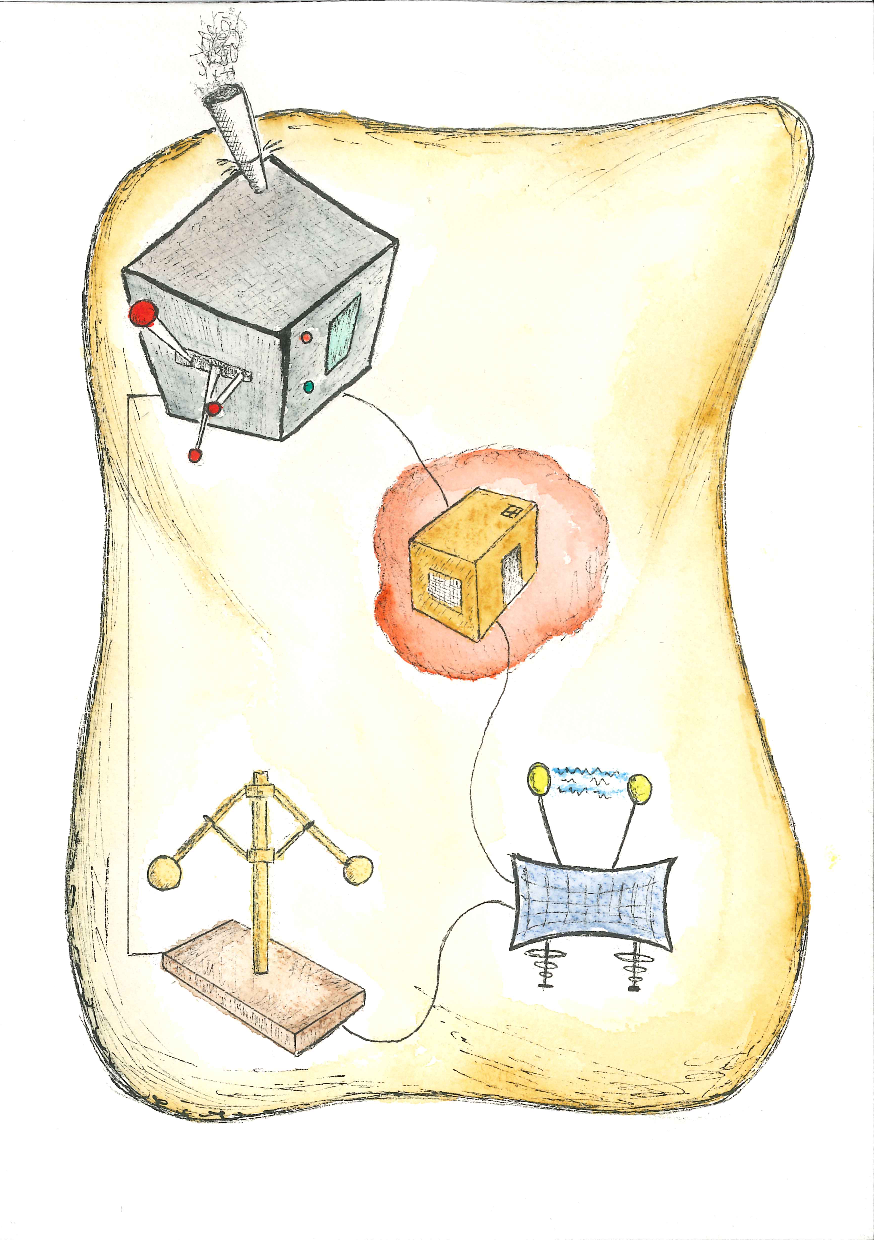
\includegraphics[trim={2mm, 2mm, 2mm, 2mm}, width=0.995\pagewidth]{scans/pan-3.pdf}};
    
   
    \begin{scope}[x={(image.south east)},y={(image.north west)}]
        \if\helplines1
        	\draw[help lines,xstep=.1,ystep=.1] (0,0) grid (1,1);
        \fi
        %\node(title) at (0.5, 0.9) {\Huge {Proteins as machines}};
        \node[align=center, anchor=north, text width=0.4\pagewidth](en) at (0.67, 0.815) {\english{\Large Proteins are the fundamental machines of the cell, and at the same time, the workers that direct them.}};
        \node[align=center, anchor=north, text width=0.3\pagewidth](es) at (0.27, 0.55) {\spanish{ \Large Las proteínas son las maquinaria fundamental de las células, y al mismo tiempo, los obreros que las accionan.}};
    \end{scope}

\end{tikzpicture}
\end{center}